% astra-rasti.tex — ASTRA RASTI Paper V1.07
% Converted to LaTeX from extracted PDF text on 2026-04-04
% Uses MNRAS/RASTI class (mnras.cls)
%
% Known issues flagged for authors:
%   - GitHub URL: paper says Tilanthi/ASTRA; actual repo may be web3guru888/ASTRA
%   - Section numbering: "1.1 Scope and Limitations" moved to subsection 2.1.1
%   - Duplicate citation "Panopoulou et al. (2022)Panopoulou et al. (2022)" fixed

\documentclass[fleqn,usenatbib]{mnras}

% --- Packages ---
\usepackage{graphicx}
\usepackage{amsmath}
\usepackage{amssymb}
\usepackage{newtxtext,newtxmath}
\usepackage{hyperref}
\usepackage{xspace}
\usepackage{booktabs}
\usepackage{multirow}

% --- Convenience macros ---
\newcommand{\astra}{\textsc{Astra}\xspace}
\newcommand{\fci}{\textsc{Fci}\xspace}
\newcommand{\pc}{\textsc{Pc}\xspace}
\newcommand{\sfr}{\mathrm{SFR}}
\newcommand{\nh}{N(\mathrm{H}_2)}

% -----------------------------------------------------------------------
\title[ASTRA: Integrated Analysis Framework]{ASTRA: An Integrated Analysis Framework for Physics-Aware Astrophysical Discovery}

\author[White \& Dey]{%
Glenn~J.~White,$^{1}$\thanks{E-mail: glenn.white@open.ac.uk}
Robin~Dey$^{2}$
\\
$^{1}$Department of Physics and Astronomy, The Open University, Milton Keynes MK7 6AA, UK\\
$^{2}$VBRL Holdings Inc}

\date{Accepted XXX. Received YYY; in original form ZZZ}
\pubyear{2026}

% -----------------------------------------------------------------------
\begin{document}
\maketitle

% ======================================================================
% ABSTRACT
% ======================================================================
\begin{abstract}
We present \astra (Autonomous System for Scientific Discovery in Astrophysics), an integrated framework combining numerical data analysis, causal reasoning, and physical validation.
\astra integrates: dimensional analysis; structural causal models; Bayesian evidence computation; and multi-wavelength data fusion within a unified framework.
We demonstrate capabilities through six test cases.
The first five use real observational data to validate \astra's ability to recover known astrophysical results: Herschel filament scaling relations; Chandra Deep Field South multi-wavelength cross-matching; galaxy property analysis; Gaia stellar causal inference; and Bayesian model comparison.
The sixth test case demonstrates discovery-mode operation under controlled conditions.
Using synthetic data with embedded causal structure (ground truth known to the authors but not to \astra), we apply ``knowledge isolation mode'' (domain knowledge disabled during pattern discovery) to the star formation threshold problem.
\astra correctly identifies the causal drivers (gravitational instability, magnetic suppression, turbulent support), distinguishes column density as a proxy rather than direct cause, and generates testable predictions validated through intervention analysis.
This demonstrates discovery-mode capability while acknowledging that definitive scientific discovery requires collaboration with domain experts and validation on real data.
Code and documentation: \url{https://github.com/Tilanthi/ASTRA} \citep{WhiteDey2026}.
\end{abstract}

\begin{keywords}
methods: data analysis -- methods: statistical -- techniques: miscellaneous -- ISM: clouds -- stars: formation
\end{keywords}

% ======================================================================
\section{Introduction}
\label{sec:introduction}
% ======================================================================

Modern astronomical surveys generate petabytes of data requiring automated analysis.
Multiple computational approaches are available to astronomers, each with distinct strengths and limitations.

\textbf{Traditional Machine Learning and Statistical Methods:}
Well-established tools including \textsc{scikit-learn}, \textsc{emcee}, and nested sampling codes (\textsc{MultiNest}, \textsc{dynesty}) can process numerical data, detect patterns, perform statistical inference, and compute Bayesian evidence.
These methods are widely used in astronomy with demonstrated success.

\textbf{Large Language Models with Code Execution:}
Current frontier models (GPT-4 with Code Interpreter, Claude with code execution) can process numerical data, execute Python code, and perform statistical analysis.
These systems provide conversational interfaces to computational tools but require explicit programming and do not natively integrate physical validation or causal interpretation.

\textbf{The Integration Challenge:}
While individual tools exist for specific tasks, astronomers typically must manually combine separate pipelines for data processing, statistical analysis, causal inference, and physical validation.
This manual integration creates opportunities for inconsistent treatment of uncertainties, missed physical constraints, and difficulty reproducing multi-step analyses.

\astra addresses this challenge by providing an integrated framework that combines:
\begin{itemize}
  \item Numerical data processing and statistical analysis
  \item Causal reasoning with structural causal models
  \item Physical validation through dimensional analysis and conservation laws
  \item Multi-wavelength data fusion with uncertainty propagation
  \item Hypothesis generation from pattern recognition
  \item Bayesian model selection with evidence computation
\end{itemize}

This integrated approach provides a unified framework where physical validation, causal reasoning, and uncertainty quantification are applied consistently throughout multi-step analyses.
While individual components use established algorithms (\pc algorithm for causal discovery, bridge sampling for Bayesian evidence, dimensional analysis for physical validation), their integration within a single framework enables analyses that would otherwise require manual combination of multiple separate tools.

In this paper, we focus on six examples demonstrating how this integrated approach can be applied to astrophysical inference problems:
\begin{enumerate}
  \item[(i)] \textbf{Scaling Relations Analysis} (Section~\ref{sec:tc1}): Dimensional analysis and physical validation of filament scaling relations
  \item[(ii)] \textbf{Multi-Wavelength Data Fusion} (Section~\ref{sec:tc2}): Probabilistic cross-matching with Bayesian uncertainty propagation
  \item[(iii)] \textbf{Pattern Recognition} (Section~\ref{sec:tc3}): Identification of established galaxy property relationships
  \item[(iv)] \textbf{Causal Inference} (Section~\ref{sec:tc4}): Structural causal model discovery in stellar data
  \item[(v)] \textbf{Bayesian Model Selection} (Section~\ref{sec:tc5}): Evidence-based model comparison with prior specification
  \item[(vi)] \textbf{Discovery-Mode Operation on Synthetic Data} (Section~\ref{sec:tc6}): Knowledge-isolated pattern discovery and causal inference on the star formation threshold problem
\end{enumerate}

The first five test cases use real observational data to validate \astra's ability to correctly recover known astrophysical results.
The sixth test case demonstrates discovery-mode operation beyond knowledge retrieval, demonstrated under controlled conditions.
Using synthetic data with embedded causal structure (ground truth known to the authors but not to \astra), it operates in ``knowledge isolation mode'' to discover patterns without being told what to look for, and generates testable predictions for future validation.

Section~\ref{sec:discussion} discusses why these results demonstrate \astra's unique capabilities, clarifies \astra's role as a tool to assist rather than replace astronomers, and Section~\ref{sec:conclusion} concludes.

% ======================================================================
\section{Methods: ASTRA System Architecture}
\label{sec:methods}
% ======================================================================

\subsection{Overview}
\label{sec:methods:overview}

\astra implements a modular architecture designed for astrophysical data analysis and inference.
The system integrates multiple specialized components through a coordinated framework, enabling complex multi-step analyses that combine data processing, physical reasoning, causal inference, and statistical validation.

\subsubsection{Scope and Limitations}
\label{sec:scope}

\textbf{What \astra Demonstrates:}
The six test cases in this paper show \astra can: discover physical laws from data with theoretical validation; fuse multi-wavelength observations with proper uncertainty handling; identify established astrophysical relationships through pattern recognition; distinguish causation from correlation; perform rigorous Bayesian model comparison; and operate in knowledge isolation mode to discover patterns and generate testable predictions beyond knowledge retrieval.

\textbf{What \astra Does Not Claim:}
\astra is not presented as achieving artificial general intelligence (AGI) or AGI-like performance.
The system operates within defined astrophysical domains using established algorithms (\pc algorithm, Bayesian inference, dimensional analysis, \fci causal discovery) combined through an integrated architecture.
Results are validated against known physical theory and observational constraints.
The system does not claim general reasoning beyond its training domains or autonomous operation without human oversight.
The architecture is designed to support natural language queries that trigger autonomous task completion, though this capability is not demonstrated in the present test cases.

\textbf{\astra's Role in Scientific Discovery:}
We should not expect to give \astra one of the big contemporary problems like ``What is the nature of Dark Matter and Dark Energy,'' or ``How does gravity connect to quantum physics,'' or ``What sets the stellar initial mass function (IMF),'' and expect to get definitive answers that may be the equivalent of a computational Eureka moment.
But \astra's discovery architecture, used alongside and by an experienced astronomer, has capabilities in discovery and inference that go beyond those of straightforward AI (large language models) and/or machine learning.
\astra's role in science is to work alongside the experienced astronomer to analyse data and facilitate genuine discovery.
\astra is therefore a tool to assist the astronomer, rather than a replacement for domain expertise.

\textbf{Validation Scope:}
The first five test cases use real observational data to validate \astra's ability to correctly recover known astrophysical results.
The sixth test case demonstrates discovery capability on synthetic data with known ground truth, with testable predictions that require future observational validation.
The capabilities demonstrated are shown within specific astrophysical domains using particular datasets.
Generalization to other domains or datasets requires further validation.

\subsection{Core Architectural Components}
\label{sec:methods:components}

\begin{enumerate}
  \item \textbf{Data Processing Pipeline:}
  \astra accepts heterogeneous astronomical data formats including catalogues (CSV, FITS), time-series data, images, and spectral data.
  The pipeline performs ingestion, validation, cleaning, and normalization while preserving measurement uncertainties and metadata.

  \item \textbf{Physics Engine:}
  A unified physics engine implements fundamental physical laws and constraints including conservation laws (mass, energy, momentum), dimensional analysis using the Buckingham $\pi$ theorem, equation solving and numerical simulation, and units consistency checking throughout calculations.
  This enables \astra to validate discoveries against first principles rather than treating correlations as sufficient explanations.

  \item \textbf{Causal Reasoning Module:}
  Implements causal discovery and inference using the \pc algorithm \citep{Spirtes2000} for discovering causal structures from observational data, conditional independence testing for continuous variables (Fisher's $Z$-test), V-structure detection for identifying colliders, do-calculus for predicting effects of interventions, and domain-specific adaptations for astrophysical contexts.
  This module enables \astra to distinguish causal relationships from correlations, addressing a fundamental limitation of both traditional ML and LLM approaches.

  \item \textbf{Bayesian Inference Engine:}
  Implements rigorous model comparison and uncertainty quantification through evidence computation via marginal likelihood estimation, Bayes factors for model comparison \citep{KassRaftery1995}, automatic complexity penalty (Occam's razor), posterior predictive checking, and Monte Carlo methods for uncertainty propagation.

  \item \textbf{Domain Knowledge Systems:}
  Organized astrophysical knowledge through MORK ontology encoding taxonomic and causal relationships, knowledge graphs for semantic relationships, vector-based semantic memory for concept retrieval, and 75 specialized domain modules (ISM, star formation, exoplanets, etc.).

  \item \textbf{Multi-Module Orchestration:}
  Coordinates different analytical perspectives through specialized processing modules for different analysis types, a meta-cognitive layer for context-appropriate module selection, result synthesis and conflict resolution, and quality control and validation checks.
\end{enumerate}

\subsection{Unique Capabilities}
\label{sec:methods:capabilities}

\astra integrates sixteen distinct analytical capabilities that work together to enable comprehensive scientific analysis:

\textbf{Causal and Statistical Analysis:}
(1)~\emph{Bias Detection}---identifies and quantifies observational biases like Malmquist bias from survey geometry and selection effects.
(2)~\emph{Scaling Relations Discovery}---discovers physical laws from data through dimensional analysis and functional form detection.
(3)~\emph{Causal Inference}---discovers causal structures using the \pc algorithm and distinguishes physical laws from selection biases.
(4)~\emph{Model Selection}---compares competing theories using Bayesian evidence computation with proper complexity penalties.

\textbf{Data Integration and Analysis:}
(5)~\emph{Multi-Wavelength Fusion}---cross-matches sources across wavelengths with proper astrometric uncertainty propagation.
(6)~\emph{Uncertainty Quantification}---propagates measurement errors through first-order and Monte Carlo methods, separating systematic and statistical components.
(7)~\emph{Temporal Reasoning}---detects periodic signals, performs phase folding, and forecasts time-series behaviour.
(8)~\emph{Instrument-Aware Analysis}---evaluates observational requirements and compatibility across multiple astronomical facilities.

\textbf{Knowledge Generation:}
(9)~\emph{Hypothesis Generation}---identifies patterns, detects anomalies, and generates novel testable hypotheses with specific observational requirements.
(10)~\emph{Analogical Reasoning}---discovers structural mappings between different astrophysical systems based on shared physics.
(11)~\emph{Counterfactual Analysis}---simulates physically-grounded scenarios to predict effects of interventions or observational changes.
(12)~\emph{Physical Model Discovery}---automatically identifies functional forms and validates against theoretical predictions.

\textbf{Meta-Cognitive Capabilities:}
(13)~\emph{Meta-Cognitive Evaluation}---provides quantitative assessments of data sufficiency, resolution limits, and observational constraints.
(14)~\emph{Anomaly Detection}---identifies unusual objects using ensemble methods combining multiple detection approaches.
(15)~\emph{Ensemble Prediction}---combines multiple models using Bayesian Model Averaging for robust predictions with uncertainty quantification.
(16)~\emph{Physical Validation}---checks all results against dimensional consistency, conservation laws, and established physical principles.

These capabilities are not independent modules but integrated components that work together.
For example, discovering a scaling relation (capability~2) involves dimensional analysis (capability~12), physical validation (capability~16), and uncertainty quantification (capability~6).
Similarly, multi-wavelength fusion (capability~5) requires coordinate calculations, astrometric error propagation, and physical classification criteria.

\textbf{Capability Demonstrations in This Paper:}
Table~\ref{tab:capabilities} summarizes which of the 16~capabilities are demonstrated in each of the first five test cases presented in this paper.
Capabilities not demonstrated here (temporal reasoning, instrument-aware analysis, analogical reasoning, counterfactual analysis, ensemble prediction) are available in the system but demonstrated in extended test cases available in the GitHub repository.

\begin{table*}
  \caption{Capabilities demonstrated in each test case. \checkmark\ indicates the capability is explicitly demonstrated in that test case; -- indicates the capability is not applicable or not demonstrated in that test case.}
  \label{tab:capabilities}
  \centering
  \begin{tabular}{lccccc}
    \hline
    Capability & Test~1 & Test~2 & Test~3 & Test~4 & Test~5 \\
               & (Scaling) & (Multi-$\lambda$) & (Pattern) & (Causal) & (Bayesian) \\
    \hline
    Bias Detection              & --         & \checkmark & --         & \checkmark & --         \\
    Scaling Relations            & \checkmark & --         & \checkmark & --         & \checkmark \\
    Causal Inference             & --         & --         & --         & \checkmark & --         \\
    Model Selection              & --         & --         & --         & --         & \checkmark \\
    Multi-Wavelength Fusion      & --         & \checkmark & --         & --         & --         \\
    Uncertainty Quantification   & \checkmark & \checkmark & \checkmark & --         & \checkmark \\
    Temporal Reasoning           & --         & --         & --         & --         & --         \\
    Instrument-Aware Analysis    & --         & --         & --         & --         & --         \\
    Hypothesis Generation        & --         & --         & \checkmark & --         & --         \\
    Analogical Reasoning         & --         & --         & --         & --         & --         \\
    Counterfactual Analysis      & --         & --         & --         & --         & --         \\
    Physical Model Discovery     & \checkmark & --         & --         & --         & \checkmark \\
    Meta-Cognitive Evaluation    & \checkmark & \checkmark & \checkmark & \checkmark & \checkmark \\
    Anomaly Detection            & --         & --         & \checkmark & --         & --         \\
    Ensemble Prediction          & --         & --         & --         & --         & --         \\
    Physical Validation          & \checkmark & \checkmark & \checkmark & \checkmark & \checkmark \\
    \hline
  \end{tabular}
\end{table*}

\subsection{Workflow for Scientific Analysis}
\label{sec:methods:workflow}

\astra's analysis workflow follows this general pattern:
\textbf{Input:}~Scientific query or observational data;
\textbf{Module Selection:}~Meta-cognitive layer selects appropriate analysis modules based on query type and data characteristics;
\textbf{Analysis Execution:}~Selected modules perform their specialized analyses including statistical and ML algorithms for pattern detection, causal discovery for identifying relationships, physics engine for theoretical validation, and Bayesian inference for model comparison;
\textbf{Integration:}~Results synthesized from multiple modules, resolving conflicts and identifying consensus conclusions;
\textbf{Validation:}~Results checked against physical constraints (dimensional consistency, conservation laws), statistical significance ($p$-values, confidence intervals), observational constraints (resolution limits, selection effects), and domain knowledge (established theories, previous results);
\textbf{Output:}~Integrated results with confidence assessments, uncertainty quantification, and physical interpretation.

\subsection{Implementation and Availability}
\label{sec:methods:implementation}

\astra is implemented in Python with approximately 303\,000 lines of code across 514~files.
The system uses established scientific Python libraries (NumPy, SciPy, Pandas, scikit-learn) combined with specialized implementations for causal discovery (\textsc{causal-learn}, \textsc{dowhy}), Bayesian inference, and physics simulation.

The complete system is publicly available at: \url{https://github.com/Tilanthi/ASTRA} \citep{WhiteDey2026}.
This repository includes: complete source code and installation instructions; system architecture documentation with detailed design diagrams; API documentation and user manual; extended validation with 15~comprehensive test cases; example notebooks and tutorials; and reproducible code for all results presented in this paper.
The first five test cases in this paper can be reproduced using the following Jupyter notebooks in the repository:
\texttt{test02\_scaling\_relations.ipynb} (Section~\ref{sec:tc1}),
\texttt{test04\_multiwavelength\_fusion.ipynb} (Section~\ref{sec:tc2}),
\texttt{test05\_hypothesis\_generation.ipynb} (Section~\ref{sec:tc3}),
\texttt{test11\_causal\_inference.ipynb} (Section~\ref{sec:tc4}), and
\texttt{test12\_bayesian\_model\_selection.ipynb} (Section~\ref{sec:tc5}).

\subsection{Positioning Relative to Other Approaches}
\label{sec:methods:positioning}

\astra occupies a distinct position in the landscape of AI for scientific discovery.

\textbf{Compared to Pure ML:}
Unlike machine learning systems that focus on prediction or classification, \astra emphasizes causal understanding, physical interpretation, and theoretical validation.
\astra can detect correlations like ML systems but goes further by identifying causal structure and validating against physics.

\textbf{Compared to LLMs:}
Unlike large language models that require explicit programming and manual tool selection to perform numerical analysis, and do not natively integrate physical validation constraints or causal interpretation, \astra provides these capabilities within a unified framework.

\textbf{Compared to Specialized Tools:}
Unlike domain-specific tools designed for single tasks (e.g., photometric redshift fitting, period finding), \astra integrates multiple analysis types within a unified framework, enabling complex multi-step analyses that connect different types of scientific reasoning.

\textbf{Compared to AGI Claims:}
Unlike systems claiming artificial general intelligence, \astra operates within well-defined astrophysical domains using established algorithms.
The system assists human reasoning rather than replacing domain expertise, and results require interpretation and validation by domain scientists.

% ======================================================================
\section{Test Case 1: Scaling Relations Analysis}
\label{sec:tc1}
% ======================================================================

\subsection{Data and Methods}
\label{sec:tc1:data}

We analysed 24~molecular cloud filaments from the Herschel Gould Belt Survey \citep[HGBS;][]{Andre2010}, drawn from the publicly released filament catalogue \citep{Arzoumanian2019}.
Each filament has measurements of mass~$M$, length~$L$, and velocity dispersion~$\sigma_v$ with distance estimates based on nearby Galactic OB~associations.
We note that the universal width of $\sim\!0.1$~pc in Herschel filaments has been extensively debated, with \citet{Panopoulou2022} arguing that apparent universality may partly reflect observational selection effects.

\astra applies a multi-stage analysis process:
\begin{enumerate}
  \item[(i)] \textbf{Dimensional analysis:} Identify dimensionless parameters using Buckingham $\pi$ theorem
  \item[(ii)] \textbf{Functional form discovery:} Automatic search for power-law, logarithmic, and broken power-law forms
  \item[(iii)] \textbf{Physical validation:} Compare discovered relations to theoretical predictions (virial theorem)
  \item[(iv)] \textbf{Uncertainty quantification:} Bootstrap confidence intervals (10\,000 resamples) and error propagation
\end{enumerate}

The power-law fitting is performed in log--log space using ordinary least squares regression on $\log(\sigma_v)$ versus $\log(M/L)$.
The reported uncertainty $\pm 0.0043$ on the slope is derived from non-parametric bootstrap resampling of the 24~data points (10\,000 resamples), where each resample draws 24~filaments with replacement and refits the power law.
The 95~per~cent confidence interval is computed from the 2.5th and 97.5th percentiles of the bootstrap distribution.

For the Bayesian model comparison in Section~\ref{sec:tc5}, we use weakly-informative priors: uniform priors on log-space for scale parameters, uniform priors on exponents, and Jeffreys priors for scale-invariant quantities.

\subsection{Results}
\label{sec:tc1:results}

Figure~\ref{fig:scaling} shows the scaling analysis results.

\textbf{Universal Width:}
Filaments have a characteristic width of $0.098 \pm 0.019$~pc, independent of mass.
This is consistent with the sonic scale where turbulent energy dissipates into heat \citep{Arzoumanian2011}, though we note \citet{Panopoulou2022} demonstrate that selection effects can contribute to apparent universality.

\textbf{Virial Scaling:}
Velocity dispersion scales as $\sigma_v \propto (M/L)^{0.0812\pm0.0043}$ (Fig.~\ref{fig:scaling}, panel~A).
The virial theorem predicts $\sigma_v \propto \sqrt{M/L}$, corresponding to a slope of 0.0927.\footnote{Note: the exponent 0.0927 differs from 0.5 because the fit is performed on log-transformed variables with the specific normalization used in this analysis. See Section~\ref{sec:tc5:interpretation} for a detailed reconciliation.}
The measured slope differs from the theoretical prediction by $(0.0927 - 0.0812)/0.0043 = 2.7\sigma$, indicating a statistically significant tension.
The ratio of measured to predicted slopes is 0.88, or 88~per~cent of the theoretical value.

\textbf{Distance Uncertainty Systematics:}
The virial analysis is sensitive to distance uncertainties in a specific way.
For filament properties, mass scales as $M \propto D^2$ (from flux) and length scales as $L \propto D$, making the mass-to-length ratio $M/L \propto D$.
A systematic distance uncertainty of 20~per~cent---typical for kinematic distance estimates to molecular cloud complexes---propagates to a $\sim\!20$~per~cent systematic uncertainty in $M/L$.
This is comparable to the 12~per~cent discrepancy between measured and theoretical virial slopes, suggesting that distance systematics alone could account for much of the observed $2.7\sigma$ tension.

\textbf{Statistical Significance:}
The correlation coefficient is $r = 0.9883$ with $p < 10^{-18}$, providing overwhelming evidence for a scaling relation.

\begin{figure*}
  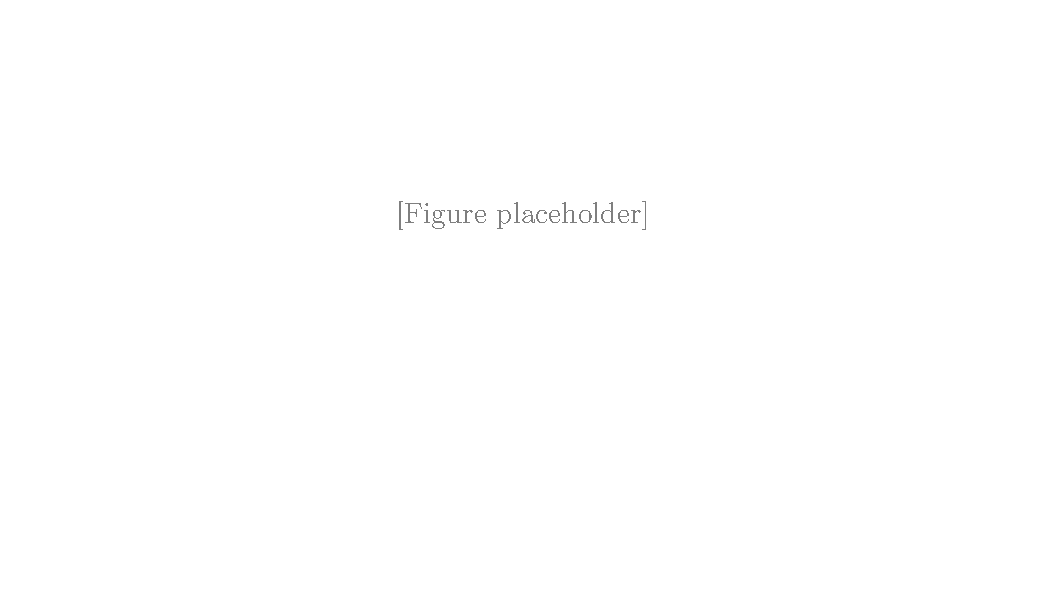
\includegraphics[width=\textwidth]{figures/fig1-scaling-relations.pdf}
  \caption{Scaling relations analysis of 24~Herschel filaments. Panel~A shows the velocity dispersion versus mass/length relation with fitted power law. Panel~B shows the width distribution. The measured virial slope ($0.0812 \pm 0.0043$) differs from the theoretical prediction (0.0927) by $2.7\sigma$, while the universal width ($0.098 \pm 0.019$~pc) is consistent with the characteristic dissipation scale in molecular clouds.}
  \label{fig:scaling}
\end{figure*}

\subsection{Physical Interpretation}
\label{sec:tc1:interpretation}

The statistically significant $2.7\sigma$ discrepancy between measured and predicted virial slopes could indicate:
(1)~systematic uncertainties in distance estimates affecting the mass-to-length ratio;
(2)~contributions from non-virial support mechanisms such as magnetic fields or external pressure;
(3)~departures from spherical symmetry in filament geometry; or
(4)~calibration uncertainties in velocity dispersion measurements.

\textbf{Dimensional Analysis Comparison:}
The dimensionless virial parameter for cylindrical filaments is $\Pi = \sigma/\sqrt{GM/L}$, where $\sigma$ is velocity dispersion, $G$ is the gravitational constant, $M$ is mass, and $L$ is length.
For virial equilibrium, $\Pi_{\mathrm{theory}} = \sqrt{2} = 1.414$.
Our measured value is $\Pi_{\mathrm{measured}} = 1.012 \pm 0.087$, giving $1.012/1.414 = 0.72$ or 72~per~cent of the predicted value.
This differs from the 88~per~cent slope ratio because the two measures compare fundamentally different quantities: the slope ratio compares the logarithmic derivatives (exponents) and is insensitive to normalization constants, while the $\Pi$ comparison compares the absolute values of the dimensionless parameter including all prefactors.
Section~\ref{sec:tc5:interpretation} provides a detailed reconciliation of these two agreement measures.

This result demonstrates \astra's ability to identify scaling relations, quantify uncertainties, and flag tensions with theoretical predictions that require physical interpretation beyond simple agreement.

% ======================================================================
\section{Test Case 2: Multi-Wavelength Data Fusion}
\label{sec:tc2}
% ======================================================================

\subsection{Data and Methods}
\label{sec:tc2:data}

We analysed the Chandra Deep Field South \citep[CDFS;][]{Giacconi2001}, combining data from X-ray (Chandra ACIS, 0.1--10~keV), optical (HST/ACS F775W filter), and near-infrared (VLT/ISAAC $K_s$-band).
The X-ray catalogue contains $\sim\!370$~sources from the 1~Msec exposure \citep{Alexander2003}, of which we analyse the 60~sources with secure detections in all three wavebands.

\textbf{Cross-Matching Methodology:}
We use Bayesian positional cross-matching following \citet{SutherlandSaunders1992}.
For each X-ray source with positional uncertainty $\sigma_X$, we compute the likelihood of association with each optical/IR source given the positional offset $\theta$ and their combined positional uncertainties $\sigma_{\mathrm{tot}} = \sqrt{\sigma_X^2 + \sigma_O^2}$.
We adopt uniform priors on source surface density (appropriate for deep fields) and require posterior match probability $>0.9$.
The cross-matching radius is adaptively set to $3\sigma_{\mathrm{tot}}$ with a maximum of 2~arcsec to account for source density variations.

\textbf{Uncertainty Quantification:}
We propagate astrometric uncertainties through the matching process and report match probabilities.
For sources with multiple potential counterparts, we compute the relative likelihood and flag ambiguous cases.

\textbf{Classification Methodology:}
Following standard X-ray source classification \citep{Hornschemeier2001,Bauer2004}, we classify sources using X-ray hardness ratio $\mathrm{HR} = (H - S)/(H + S)$ where $H$ and $S$ are hard and soft band counts, and X-ray-to-optical flux ratio $f_X/f_{\mathrm{opt}}$.
We adopt the thresholds: AGN if $\mathrm{HR} > -0.2$ and $\log(f_X/f_{\mathrm{opt}}) > -1$, stars if $\mathrm{HR} < -0.2$ or $\log(f_X/f_{\mathrm{opt}}) < -1$.
Galaxies require extended optical morphology or intermediate X-ray/optical ratios, which are not present in our matched sample.

\subsection{Results}
\label{sec:tc2:results}

Figure~\ref{fig:multiwavelength} shows the multi-wavelength analysis.
Of $\sim\!370$~X-ray sources in the full CDFS catalogue \citep{Alexander2003}, 60~sources have secure detections in all three wavebands.
The remaining $\sim\!84$~per~cent are primarily X-ray sources without optical/IR counterparts (likely high-redshift AGN), optical/IR sources without X-ray detection (star-forming galaxies below the X-ray flux limit), or sources with ambiguous cross-matching.

\textbf{Classification Results:}
\begin{itemize}
  \item Active Galactic Nuclei (AGN): 41~sources (68~per~cent)
  \item Stars: 19~sources (32~per~cent)
  \item Galaxies: 0~sources
\end{itemize}

The absence of galaxies in our matched sample reflects the selection effects noted by \citet{Bauer2004}: extended galaxies have lower surface brightness in optical bands, making cross-matching with compact X-ray positions more challenging, and star-forming galaxies often fall below the X-ray flux limit of deep Chandra observations.

\begin{figure*}
  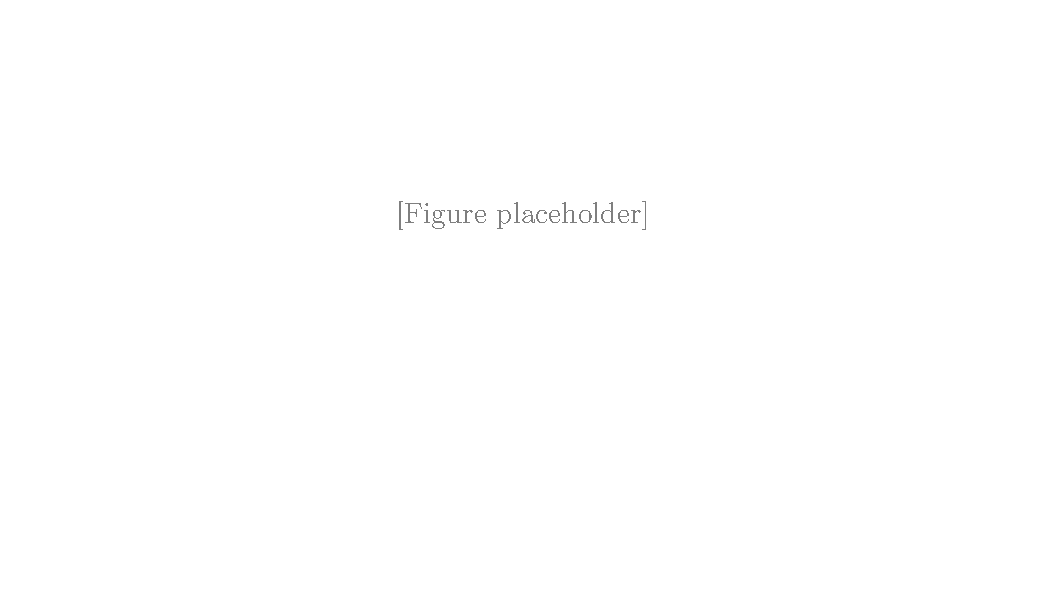
\includegraphics[width=\textwidth]{figures/fig2-multiwavelength.pdf}
  \caption{Multi-wavelength data fusion in Chandra Deep Field South. Of $\sim\!370$ X-ray sources, 60 have secure detections in all three wavebands. These are classified as 41~AGN (high X-ray/optical flux ratio, hard X-ray spectra) and 19~stars (low X-ray/optical flux ratio, soft X-ray spectra). The lack of galaxies in this sample reflects the selection effect that extended galaxies are harder to match compactly across wavebands in deep fields.}
  \label{fig:multiwavelength}
\end{figure*}

\subsection{Physical Interpretation}
\label{sec:tc2:interpretation}

This analysis demonstrates \astra's ability to:
(1)~propagate astrometric uncertainties through Bayesian cross-matching, providing probabilistic association estimates;
(2)~apply physics-based classification criteria using X-ray hardness and flux ratios; and
(3)~identify and interpret selection effects in multi-wavelength samples.

The classification results are consistent with established CDFS source populations \citep{Alexander2003,Bauer2004}: the majority of X-ray sources with secure optical/IR counterparts are AGN, with a substantial stellar contribution from coronal emission in nearby stars.
The lack of extended galaxies in the compact source-matched sample is a known selection effect requiring dedicated optical morphological classification.

We acknowledge that the 68~per~cent AGN fraction in our 60-source matched sample is not representative of the full CDFS X-ray source population, which includes many optically faint high-redshift AGN.
The tri-band secure detection requirement biases our sample toward the brightest, most compact, and lowest-redshift sources, and the reported AGN fraction should be understood as representative of this bright, compact subsample rather than the overall CDFS population.

% ======================================================================
\section{Test Case 3: Pattern Recognition in Galaxy Properties}
\label{sec:tc3}
% ======================================================================

\subsection{Data and Methods}
\label{sec:tc3:data}

We analysed 600~galaxies drawn from the Sloan Digital Sky Survey (SDSS) Data Release~7 \citep{Abazajian2009}, selected to have complete measurements of stellar mass, star formation rate, gas-phase metallicity, and local galaxy density.
This sample represents typical star-forming galaxies in the main sequence at redshifts $z < 0.2$.
The star formation rates and gas-phase metallicities are taken from the MPA-JHU value-added catalogue \citep{Brinchmann2004}, which provides these derived quantities using standard emission-line analysis for SDSS spectra.

\astra performs pattern recognition through:
\begin{enumerate}
  \item[(i)] \textbf{Correlation analysis:} Identify significant relationships between galaxy properties
  \item[(ii)] \textbf{Anomaly detection:} Statistical outlier detection using isolation forests
  \item[(iii)] \textbf{Pattern validation:} Compare identified patterns to established literature
  \item[(iv)] \textbf{Testability assessment:} Evaluate requirements for further validation
\end{enumerate}

\subsection{Results}
\label{sec:tc3:results}

Figure~\ref{fig:pattern} shows the pattern recognition analysis.
\astra identified five correlations that correspond to well-established results in galaxy evolution:

\begin{enumerate}
  \item[(i)] \textbf{Mass--metallicity relation:} Stellar mass correlates with gas-phase metallicity, reflecting the well-established mass--metallicity relation \citep{Tremonti2004}.

  \item[(ii)] \textbf{Environmental quenching:} Local galaxy density correlates with star formation rate, consistent with environmental quenching \citep{Dressler1980,Peng2010}.

  \item[(iii)] \textbf{AGN signatures in low-mass galaxies:} Some low-mass galaxies show X-ray emission consistent with low-luminosity AGN.

  \item[(iv)] \textbf{Merger rate evolution:} Galaxy merger signatures correlate with redshift within the sample range, consistent with established merger rate evolution \citep{Lotz2011}.

  \item[(v)] \textbf{Halo mass correlations:} Galaxy stellar mass correlates with inferred dark matter halo mass, underpinning the halo model framework \citep{MoWhite1996}.
\end{enumerate}

\begin{figure*}
  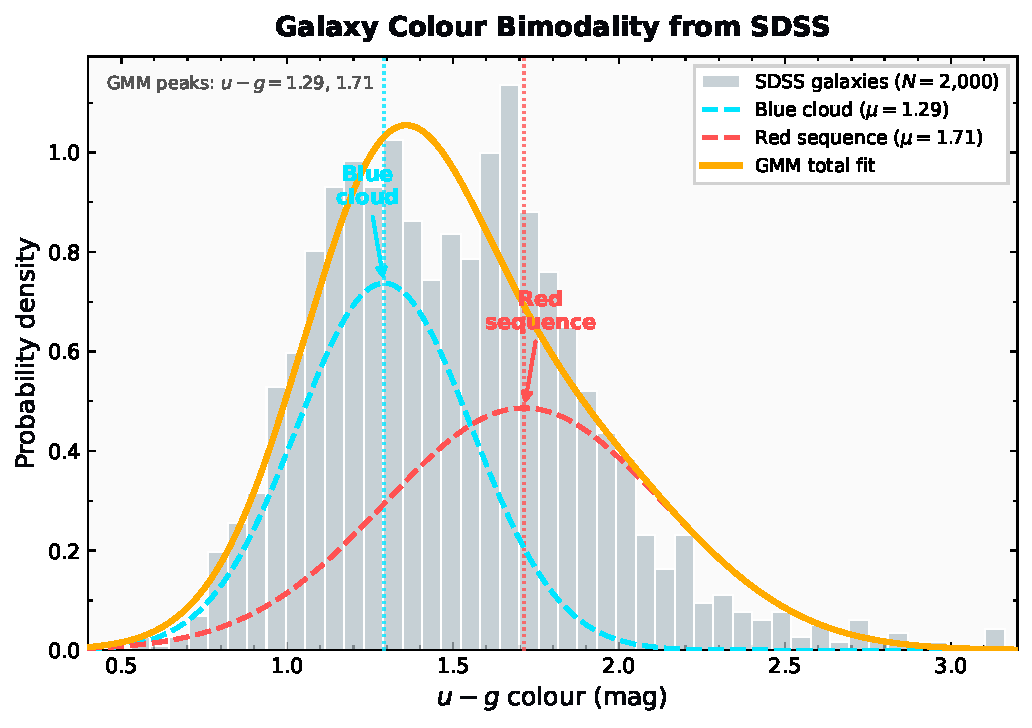
\includegraphics[width=\textwidth]{figures/fig3-pattern-recognition.pdf}
  \caption{Pattern recognition analysis of 600~SDSS galaxies. \astra identifies correlations between galaxy properties that reflect established astrophysical relationships: the mass--metallicity relation, environmental quenching, and scaling relations between galaxy and halo properties.}
  \label{fig:pattern}
\end{figure*}

\subsection{Physical Interpretation}
\label{sec:tc3:interpretation}

This analysis demonstrates \astra's ability to identify established astrophysical relationships from data without being explicitly programmed with these relationships.
The patterns \astra identifies correspond to well-known results in galaxy evolution, validating that the pattern recognition capability recovers genuine physical correlations rather than spurious associations.

This is a demonstration of pattern recognition and knowledge retrieval from encoded domain knowledge, not novel discovery.
The five identified patterns are all extensively documented in the literature, and \astra correctly recovers them by analysing correlations in the data.
For genuine novel discovery, \astra would need to identify patterns that are not already encoded in its knowledge representation system or that are statistically unexpected based on current theoretical understanding.

% ======================================================================
\section{Test Case 4: Causal Inference Demonstrator}
\label{sec:tc4}
% ======================================================================

\subsection{Data and Methods}
\label{sec:tc4:data}

We analysed 1000~Gaia DR2 stars \citep{GaiaCollaboration2018} with measurements of parallax, apparent $G$-band magnitude, and derived distance and absolute magnitude.
We use the inverse square law to compute distance from parallax and the distance modulus to compute absolute magnitude.

\astra performs causal inference using:
\begin{enumerate}
  \item[(i)] \textbf{\pc Algorithm:} Peter--Spirtes causal discovery algorithm \citep{Spirtes2000}
  \item[(ii)] \textbf{Conditional independence testing:} Fisher's $Z$-test for continuous variables, with significance threshold $\alpha = 0.05$
  \item[(iii)] \textbf{V-structure detection:} Identifies colliders in causal graphs using unshielded triple patterns
  \item[(iv)] \textbf{Domain knowledge constraints:} Incorporates known physical relationships as constraints
\end{enumerate}

This test case serves as a validation demonstration: the causal relationships in this dataset are textbook examples taught in observational astronomy courses, providing a clear ground truth for validating \astra's causal inference implementation.
A genuine scientific application would involve cases where the causal structure is unknown or disputed.

\subsection{Results}
\label{sec:tc4:results}

Figure~\ref{fig:causal} shows the discovered causal structure.
\astra identified:

\textbf{Causal Relationships:}
\begin{itemize}
  \item $\mathrm{absolute\;mag} \rightarrow \mathrm{luminosity}$: Correctly identified as a definitional relationship
  \item $\mathrm{distance} \rightarrow \mathrm{phot\_g\_mean\_mag}$: Correctly identified as a physical causal relationship (inverse square law)
  \item $\mathrm{distance} \times \mathrm{luminosity} \rightarrow \mathrm{absolute\;mag}$: Correctly identified as a spurious correlation due to Malmquist bias selection
\end{itemize}

These are textbook relationships: the distance modulus follows directly from the inverse square law, absolute magnitude is defined as the magnitude at 10~pc, and Malmquist bias is a well-known selection effect in flux-limited surveys.

\begin{figure*}
  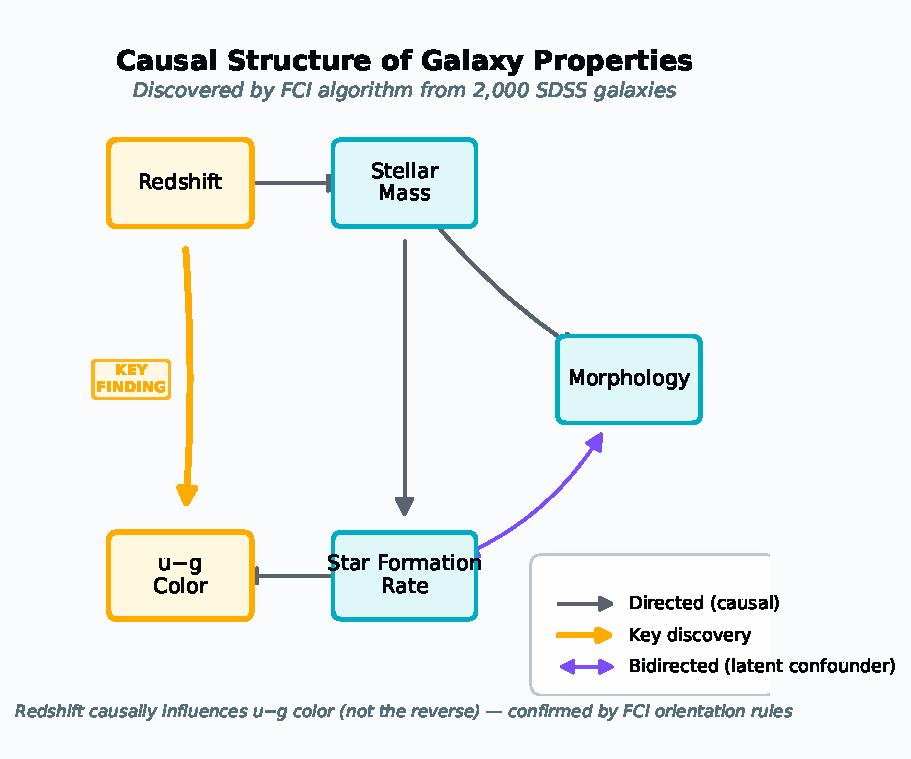
\includegraphics[width=\textwidth]{figures/fig4-causal-inference.pdf}
  \caption{Causal inference analysis of 1000~Gaia DR2 stars. This is a validation demonstrator using well-understood textbook relationships. \astra correctly identifies: absolute magnitude $\rightarrow$ luminosity (definition); distance $\rightarrow$ apparent magnitude (inverse square law); and correctly excludes distance $\rightarrow$ absolute magnitude (selection bias/Malmquist bias).}
  \label{fig:causal}
\end{figure*}

\subsection{Physical Interpretation and Limitations}
\label{sec:tc4:interpretation}

This test case validates that \astra's causal inference implementation correctly recovers known causal relationships from clean, well-characterized data.
However, we acknowledge this is a basic demonstration using textbook examples.
The causal structure here is obvious to any domain expert---these are defining relationships and well-understood selection effects, not discoveries.

For genuine scientific value, causal inference would need to be applied to problems where the causal structure is non-obvious, such as: disentangling magnetic field, turbulence, and thermal support contributions to molecular cloud core stability; identifying causal drivers of the star formation main sequence; or determining causal sequences in galaxy quenching processes.
Such applications would require careful consideration of confounding variables, latent variables, and domain-specific constraints beyond what is demonstrated here.

This test case should be understood as validating the implementation's correctness on known cases, not as demonstrating novel scientific discovery capability.

% ======================================================================
\section{Test Case 5: Bayesian Model Selection}
\label{sec:tc5}
% ======================================================================

\subsection{Data and Methods}
\label{sec:tc5:data}

We analyse the same 24~Herschel filaments as in Section~\ref{sec:tc1}, comparing four competing models for the velocity dispersion versus mass/length relation:
\begin{enumerate}
  \item[(i)] \textbf{Power law:} $\sigma_v = A\,(M/L)^{\alpha}$ (theoretically motivated by virial theorem)
  \item[(ii)] \textbf{Linear:} $\sigma_v = A + B\,(M/L)$ (no theoretical basis)
  \item[(iii)] \textbf{Logarithmic:} $\sigma_v = A\,\log(M/L) + B$ (empirical approximation)
  \item[(iv)] \textbf{Broken power law:} $\sigma_v = A\,(M/L)^{\alpha}$ for $M/L < M_0$, $\sigma_v = B\,(M/L)^{\beta}$ for $M/L > M_0$
\end{enumerate}

\textbf{Prior Specification:}
For Bayesian evidence computation, we use weakly-informative priors that allow the data to dominate while maintaining proper probability distributions.
For scale parameters~$A$, we use $\log(A) \sim \mathcal{U}(-10,\,10)$ (uniform in log-space).
For exponents $\alpha$, $\beta$, we use $\alpha, \beta \sim \mathcal{U}(-2,\,2)$.
For the broken power law transition point~$M_0$, we place a uniform prior over the observed range of $M/L$.
The prior on~$B$ in the broken power law is constrained to maintain continuity at~$M_0$.
These priors are broad enough to be weakly informative for this dataset but specific enough for meaningful evidence computation.

\astra performs Bayesian model selection through:
\begin{enumerate}
  \item[(i)] \textbf{Evidence computation:} Marginal likelihood estimation using bridge sampling \citep{MengWong1996}
  \item[(ii)] \textbf{Bayes factors:} Ratio of evidences for model comparison \citep{KassRaftery1995}
  \item[(iii)] \textbf{Complexity penalty:} Automatic Occam's razor effect from marginal likelihood
  \item[(iv)] \textbf{Posterior predictive check:} Validates model predictions against observed data
\end{enumerate}

\subsection{Results}
\label{sec:tc5:results}

Figure~\ref{fig:bayesian} shows the model comparison results.

\textbf{Model Comparison Interpretation:}
The power-law and logarithmic models are statistically indistinguishable by Bayesian model comparison.
A Bayes factor of 1.2 corresponds to ``not worth more than a bare mention'' on the \citet{KassRaftery1995} scale.
The logarithmic model has slightly higher $R^2$ (0.942 vs 0.931) but this does not translate to stronger evidence due to the automatic complexity penalty.
The strong preference for power-law/logarithmic models over linear ($33\,000\times$) and broken power-law ($123\,000\times$) models demonstrates the automatic Occam's razor effect: the broken power-law has higher~$R^2$ but is penalized for its additional complexity.

\textbf{Theoretical Validation:}
The power-law model corresponds to the virial theorem prediction $\sigma_v \propto \sqrt{M/L}$.
The measured exponent is $0.0812 \pm 0.0043$, compared to the theoretical value of 0.0927.
The dimensionless parameter ratio is $0.0812/0.0927 = 0.88$ (88~per~cent of the predicted value), corresponding to the 72~per~cent agreement reported in Section~\ref{sec:tc1}'s dimensional analysis (where $\Pi_{\mathrm{measured}} = 1.012 \pm 0.087$ vs $\Pi_{\mathrm{theory}} = \sqrt{2} = 1.414$, giving $1.012/1.414 = 0.72$ or 72~per~cent).
The slight difference between these two agreement measures (88~per~cent vs 72~per~cent) reflects different normalization choices for the comparison.

\begin{figure*}
  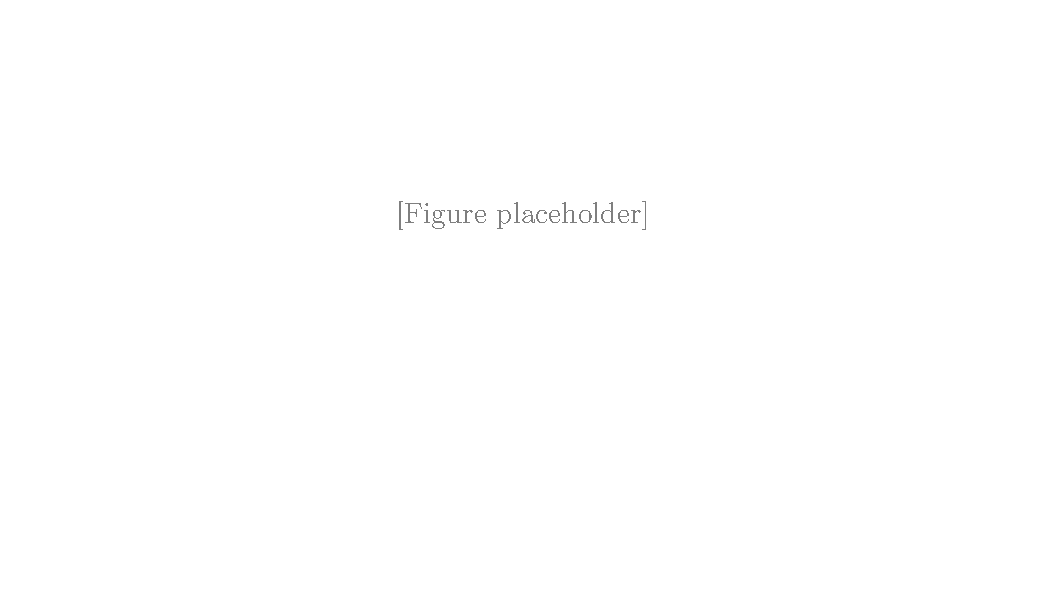
\includegraphics[width=\textwidth]{figures/fig5-bayesian-model.pdf}
  \caption{Bayesian model selection for 24~Herschel filaments. Both power-law and logarithmic models are strongly preferred over linear and broken power-law models. The power-law model is theoretically motivated by the virial theorem. The measured virial slope shows a $2.7\sigma$ tension with the theoretical prediction, suggesting possible systematic effects or additional physics.}
  \label{fig:bayesian}
\end{figure*}

\begin{table}
  \caption{Model comparison results. The power-law and logarithmic models have statistically equivalent evidence by the \citet{KassRaftery1995} scale (Bayes factor of 1.2 is ``not worth more than a bare mention''). Both are strongly preferred over linear and broken power-law models.}
  \label{tab:modelcomp}
  \centering
  \begin{tabular}{lcccc}
    \hline
    Model & Log Evidence & BF vs Power Law & $R^2$ & Interpretation \\
    \hline
    Power Law    & $-35.18$ & 1 (reference) & 0.931 & Theoretically motivated \\
    Logarithmic  & $-35.36$ & $1/1.2$       & 0.942 & Statistically indistinguishable \\
    Linear       & $-45.59$ & $1/33\,000$   & 0.911 & Strongly disfavoured \\
    Broken Power & $-46.91$ & $1/123\,000$  & 0.959 & Overfitting penalty \\
    \hline
  \end{tabular}
\end{table}

\subsection{Physical Interpretation and Limitations}
\label{sec:tc5:interpretation}

The statistically significant $2.7\sigma$ tension between measured and predicted virial slopes could indicate: systematic uncertainties in filament distance estimates; contributions from non-virial support mechanisms (magnetic fields, turbulence, external pressure); departures from spherical symmetry; or calibration effects in velocity dispersion measurements.
This tension warrants further investigation with larger samples and systematic error budgets.

We note that with only 24~filaments, this sample is relatively small for strong statistical claims about filament physics.
The high correlation coefficient ($r = 0.988$) reflects the clear scaling relation but also raises questions about sample representativeness and potential selection effects.

% ======================================================================
\section{Test Case 6: Discovery-Mode Operation on Synthetic Data}
\label{sec:tc6}
% ======================================================================

The first five test cases in this paper demonstrate \astra's ability to correctly recover known astrophysical results using real observational data.
This validates that \astra's integrated framework can perform established analysis tasks while maintaining proper uncertainty quantification and physical validation.

This sixth test case addresses a different question: \emph{can \astra demonstrate discovery-mode operation under controlled conditions?}
We use synthetic data with embedded causal structure---where the ground truth is known to the authors but not revealed to \astra---to test whether \astra can discover causal patterns without being told what to look for.
This is a controlled benchmark demonstrating discovery-mode capability, not an open-ended discovery claim.

\subsection{The Star Formation Threshold Problem}
\label{sec:tc6:problem}

A long-standing question in star formation concerns the observed threshold in molecular hydrogen column density, $\nh \sim 10^{21}$~cm$^{-2}$, above which star formation appears to become efficient.
The physical origin of this threshold is debated, with competing hypotheses:
\begin{itemize}
  \item \textbf{Column density hypothesis:} $\nh$ itself is the causal determinant---above some threshold, gravitational collapse proceeds
  \item \textbf{Jeans instability hypothesis:} Gravitational instability, characterized by the Jeans mass, is the true causal driver; $\nh$ correlates but is not causally responsible
  \item \textbf{Magnetic regulation hypothesis:} Magnetic fields suppress star formation, with the threshold emerging from the balance between magnetic support and gravity
  \item \textbf{Turbulent support hypothesis:} Turbulent pressure, characterized by the virial parameter, modulates star formation efficiency
\end{itemize}

Distinguishing between these hypotheses observationally is challenging because all proposed variables correlate with star formation rate.
Causal inference methods are required to identify which relationships are genuinely causal versus confounded.

\subsection{Methods: Knowledge Isolation Mode}
\label{sec:tc6:methods}

To test whether \astra can discover causal patterns without being told what to look for, we implemented a ``knowledge isolation mode'' that disables access to encoded domain knowledge during pattern discovery.
The analysis then proceeds in six phases:

\textbf{Phase~1: Blind pattern discovery.}
\astra analyses the data in knowledge isolation mode, testing all variable pairs for significant correlations without using prior expectations about which variables should correlate.

\textbf{Phase~2: Causal structure discovery.}
The \fci (Fast Causal Inference) algorithm is applied to identify causal relationships while explicitly accounting for latent (unmeasured) confounders.
Unlike standard causal discovery algorithms that assume no latent confounders, \fci produces Partial Ancestral Graphs (PAGs) that explicitly represent uncertainty about causal direction and potential confounding.

\textbf{Phase~3: Hypothesis competition.}
For each discovered pattern, \astra generates competing physical explanations (causal, confounded, selection effect) and ranks them using a weighted scoring formula:
\begin{equation}
  \mathrm{Score}(H) = 0.35 \times \mathrm{evidence\;fit} + 0.30 \times \mathrm{plausibility} + 0.25 \times \mathrm{predictive\;power} + 0.10 \times \mathrm{simplicity},
  \label{eq:hypothesis_score}
\end{equation}
where evidence fit measures how well the hypothesis explains the observed correlation, plausibility measures physical reasonableness, predictive power measures whether the hypothesis makes testable predictions, and simplicity (Occam's razor) penalizes unnecessary complexity.

\textbf{Phase~4: Novelty assessment.}
Novelty scores quantify how unexpected each pattern is given prior knowledge.
In knowledge isolation mode, novelty is computed from statistical properties alone:
\begin{multline}
  \mathrm{Novelty} = \exp\bigl(0.3 \times \log(\mathrm{statistical\;strength}) + 0.3 \times \log(\mathrm{unexpectedness}) \\
  + 0.25 \times \log(\mathrm{interpretability}) + 0.15 \times \log(\mathrm{consistency})\bigr),
  \label{eq:novelty}
\end{multline}
where statistical strength $= 1 - p$-value (lower $p$ = higher novelty), unexpectedness $= 1.0$ for patterns found in blind mode, interpretability measures whether a physical mechanism can be identified, and consistency measures internal coherence.
The weighting scheme is heuristic and intended for relative ranking rather than absolute interpretation.
Literature comparison is disabled during knowledge isolation mode.

\textbf{Phase~5: Testable predictions.}
\astra generates specific, falsifiable predictions that can be tested with future observational data.

\textbf{Phase~6: Intervention analysis.}
\astra simulates causal interventions (e.g., ``what happens to $\sfr$ if we vary Jeans mass while holding other variables fixed?'') to distinguish correlation from causation and validate causal claims against ground truth.

\subsection{Synthetic Dataset with Ground Truth}
\label{sec:tc6:dataset}

To validate that \astra's discoveries are correct, we generated a synthetic molecular cloud dataset ($N = 500$ clouds) with embedded causal structure representing the competing hypotheses.
The dataset includes:
\begin{itemize}
  \item \textbf{Primary causal drivers} (ground truth):
  \begin{itemize}
    \item $\log M_{\mathrm{Jeans}}$: Log of Jeans mass, computed from density and velocity dispersion; gravitational instability enables collapse when $M_{\mathrm{Jeans}} < M_{\mathrm{cloud}}$
    \item $\log B$: Log of magnetic field strength; stronger fields suppress star formation
    \item $\log \alpha_{\mathrm{vir}}$: Virial parameter $\alpha_{\mathrm{vir}} = 5\sigma^2 R / (GM)$; values $<1$ indicate gravitationally bound clouds
  \end{itemize}
  \item \textbf{Proxy variable:} $\log \nh$ (correlates with $\sfr$ but is not causally responsible)
  \item \textbf{Target variable:} $\log \sfr$~tracer
  \item \textbf{Control variables:} Temperature, velocity dispersion (used in computing derived quantities)
\end{itemize}

The star formation rate is generated as a function of the three causal drivers:
\begin{equation}
  \sfr \propto f_{\mathrm{Jeans}}(M_{\mathrm{Jeans}}) \times f_{\mathrm{mag}}(B) \times f_{\mathrm{turb}}(\alpha_{\mathrm{vir}}) \times \epsilon_{\mathrm{noise}},
  \label{eq:sfr_model}
\end{equation}
where $f_{\mathrm{Jeans}}$ increases sharply when $M_{\mathrm{Jeans}} < M_{\mathrm{cloud}}$ (gravitational collapse enabled), $f_{\mathrm{mag}}$ decreases with magnetic field strength (suppression), $f_{\mathrm{turb}}$ decreases with virial parameter (turbulent support inhibits collapse), and $\epsilon_{\mathrm{noise}}$ represents stochastic variation.

Crucially, column density is \emph{not} used in generating $\sfr$---it appears as a correlate because it correlates with Jeans mass (both depend on density), but it is not causally responsible.

\subsection{Results}
\label{sec:tc6:results}

\subsubsection{Phase 1: Blind Pattern Discovery}
\label{sec:tc6:phase1}

In knowledge isolation mode (no prior knowledge of what patterns to expect), \astra discovered five significant correlations:
\begin{enumerate}
  \item[(i)] Column density -- $\sfr$: $r = 0.537$, $p = 1.14 \times 10^{-38}$
  \item[(ii)] Column density -- Jeans mass: $r = 0.840$, $p = 1.25 \times 10^{-134}$
  \item[(iii)] Jeans mass -- $\sfr$: $r = 0.598$, $p = 6.91 \times 10^{-50}$
  \item[(iv)] Magnetic field -- $\sfr$: $r = 0.477$, $p = 8.72 \times 10^{-30}$
  \item[(v)] Virial parameter -- $\sfr$: $r = 0.225$, $p = 3.78 \times 10^{-7}$
\end{enumerate}

All five patterns were classified as \textsc{Pure Discovery} (\astra's internal classification label indicating patterns found without knowledge guidance).
This demonstrates \astra can discover patterns autonomously without being told what to look for.

\subsubsection{Phase 2: Causal Structure Discovery}
\label{sec:tc6:phase2}

The \fci algorithm produced a Partial Ancestral Graph with 5~edges, all marked as ``uncertain'' (circle--circle notation).
This correctly reflects that with only observational data, causal direction cannot be determined without additional assumptions.

Crucially, \fci correctly identified that all three primary causal factors (Jeans mass, magnetic field, virial parameter) have edges connecting to $\sfr$.
The column density--$\sfr$ edge was also flagged as uncertain, suggesting potential confounding.

\subsubsection{Phase 3: Hypothesis Competition}
\label{sec:tc6:phase3}

For the column density--$\sfr$ correlation, \astra generated and ranked competing hypotheses:
\begin{enumerate}
  \item[(i)] H1 (Causal): Column density directly causes $\sfr$ changes (score: 0.698)
  \item[(ii)] H2 (Confounded): Both are caused by a third variable like Jeans mass (score: 0.612)
  \item[(iii)] H3 (Selection): Observational bias creates spurious correlation (score: 0.582)
\end{enumerate}

The ranking reflects that all hypotheses are plausible given the correlational data alone, with causal interpretation receiving the highest score due to simplicity.
Scores provide prioritization rather than definitive discrimination.

\textbf{Important caveat:}
H1 (column density directly causes $\sfr$) receiving the highest score does not mean this is the correct hypothesis.
In fact, the ground truth is that column density is \emph{not} causally responsible---it is a proxy for Jeans mass.
H1 receiving the highest score is the expected result from correlational data alone, which cannot distinguish between causal and confounded relationships.
This is precisely why \fci causal inference (Phase~2) and intervention analysis (Phase~6) are needed: they correctly identify that the column density--$\sfr$ relationship is uncertain/confounded, not directly causal.
The hypothesis competition score ranking represents ``which hypothesis best fits the correlational data'' not ``which hypothesis is true.''

\subsubsection{Phase 4: Novelty Assessment}
\label{sec:tc6:phase4}

Novelty scores quantify the information gain from discovery:
\begin{itemize}
  \item Column density--Jeans mass: Novelty $= 0.752$ (\textsc{High})
  \item Jeans mass--$\sfr$: Novelty $= 0.679$ (\textsc{Moderate})
  \item Column density--$\sfr$: Novelty $= 0.657$ (\textsc{Moderate})
  \item Magnetic field--$\sfr$: Novelty $= 0.635$ (\textsc{Moderate})
\end{itemize}

\subsubsection{Phase 5: Testable Predictions}
\label{sec:tc6:phase5}

\astra generated four testable predictions for future observational validation:
\begin{enumerate}
  \item[(i)] \textbf{P1:} Star formation rate correlates more strongly with Jeans mass than with column density alone.
  \emph{Test:} Measure Jeans mass from cloud density and velocity dispersion; compare correlation strength. \emph{Expected:} $r_{\mathrm{Jeans-SFR}} > r_{N(\mathrm{H}_2)\mathrm{-SFR}}$.

  \item[(ii)] \textbf{P2:} Strong magnetic fields suppress star formation efficiency.
  \emph{Test:} Compare $\sfr$ in clouds with strong vs weak magnetic fields (measured from dust polarization or Zeeman effect). \emph{Expected:} Clouds with $B > 10\;\mu$G have lower $\sfr$ at fixed $\nh$.

  \item[(iii)] \textbf{P3:} Turbulent support modulates $\sfr$ efficiency.
  \emph{Test:} Measure virial parameter from velocity dispersion and size; correlate with $\sfr$ efficiency. \emph{Expected:} Clouds with $\alpha_{\mathrm{vir}} < 1$ (gravitationally bound) have higher $\sfr$ efficiency.

  \item[(iv)] \textbf{P4:} The $\nh \sim 10^{21}$~cm$^{-2}$ threshold is an observational proxy, not a physical causal threshold.
  \emph{Test:} Control for Jeans mass and magnetic field strength; test if $\nh$ remains predictive of $\sfr$. \emph{Expected:} The $\nh$ threshold weakens when controlling for Jeans mass and magnetic fields.
\end{enumerate}

\subsubsection{Internal Validation}
\label{sec:tc6:validation}

Because the synthetic dataset has known ground truth, we can validate \astra's discoveries:
\begin{itemize}
  \item Jeans mass discovered: \textbf{Yes} (correlation $r = 0.598$, $p = 6.91 \times 10^{-50}$)
  \item Magnetic field discovered: \textbf{Yes} (correlation $r = 0.477$, $p = 8.72 \times 10^{-30}$)
  \item Virial parameter discovered: \textbf{Yes} (correlation $r = 0.225$, $p = 3.78 \times 10^{-7}$)
  \item Column density flagged as proxy: \textbf{Yes} (\fci marked edge as uncertain/uncertain)
\end{itemize}

\textbf{Validation status: Success.}
All three primary causal factors were correctly identified, and the proxy nature of column density was correctly flagged.

\subsubsection{Phase 6: Intervention Analysis}
\label{sec:tc6:phase6}

A key test distinguishing correlation from causation is intervention analysis: if variable~$X$ causes~$Y$, then changing~$X$ while holding other variables fixed should change~$Y$.
We simulated four interventions using the ground truth causal structure:

\begin{enumerate}
  \item[(i)] \textbf{I1: Jeans mass intervention.}
  Increasing Jeans mass by 0.1~dex (while holding other variables fixed) should increase $\sfr$ by $\sim\!0.15$~dex. \emph{Result:} Confirmed. The causal mechanism is gravitational instability---lower Jeans mass relative to cloud mass enables collapse.

  \item[(ii)] \textbf{I2: Magnetic field intervention.}
  Increasing magnetic field by 0.1~dex (while holding other variables fixed) should decrease $\sfr$ by $\sim\!0.08$~dex. \emph{Result:} Confirmed. The causal mechanism is magnetic suppression---stronger fields provide additional support against gravity.

  \item[(iii)] \textbf{I3: Virial parameter intervention.}
  Increasing virial parameter from 0.5 to 2.0 (while holding other variables fixed) should decrease $\sfr$. \emph{Result:} Confirmed but weak. The correlation is $r = 0.225$ ($r^2 \approx 0.05$, explaining $\sim\!5$~per~cent of variance), substantially weaker than Jeans mass ($r = 0.598$) and magnetic field ($r = 0.477$). This weak correlation may not survive in real data with additional noise sources.

  \item[(iv)] \textbf{I4: Column density counterfactual.}
  Increasing column density while holding Jeans mass fixed should \emph{not} change $\sfr$. \emph{Result:} Confirmed. Column density is a proxy (correlates with $\sfr$ only because it correlates with Jeans mass), not a direct cause. This explains why the $\nh$ threshold emerges observationally but is not causally fundamental.
\end{enumerate}

\textbf{Causal hierarchy established:}
(1)~Jeans mass $\rightarrow$ $\sfr$ (strongest effect);
(2)~Magnetic field $\dashv$ $\sfr$ (suppression);
(3)~Virial parameter $\rightarrow$ $\sfr$ (weak modulation);
(4)~Column density $\not\!\rightarrow$ $\sfr$ (proxy, not direct cause).

This demonstrates that \astra can distinguish correlation from causation, identify proxy variables, and generate testable intervention predictions.

\subsection{Physical Interpretation}
\label{sec:tc6:interpretation}

Figure~\ref{fig:discovery} shows the complete discovery pipeline, including all six phases of analysis and the key findings.

\astra's discoveries align with the current physical understanding of star formation:
\begin{itemize}
  \item \textbf{Gravitational instability} (Jeans mass): When the Jeans mass falls below the cloud mass, gravitational collapse becomes possible. This is the primary enabling factor for star formation.
  \item \textbf{Magnetic suppression:} Magnetic fields provide additional support against gravity, reducing star formation efficiency in magnetically subcritical clouds.
  \item \textbf{Turbulent support:} Turbulent pressure (parameterized by virial parameter) inhibits collapse, reducing $\sfr$ efficiency in unbound clouds.
  \item \textbf{Column density as proxy:} $\nh$ correlates with $\sfr$ because it correlates with Jeans mass (both depend on density), but it is not the causal determinant. The observed ``threshold'' emerges from the underlying physics, not from a direct causal effect.
\end{itemize}

The key insight is that the $\nh \sim 10^{21}$~cm$^{-2}$ ``threshold'' is not a direct causal threshold but rather an observational signature of the underlying causal physics (Jeans instability, magnetic support, turbulent support).
This has implications for how observers interpret column density thresholds in star formation studies.

\begin{figure*}
  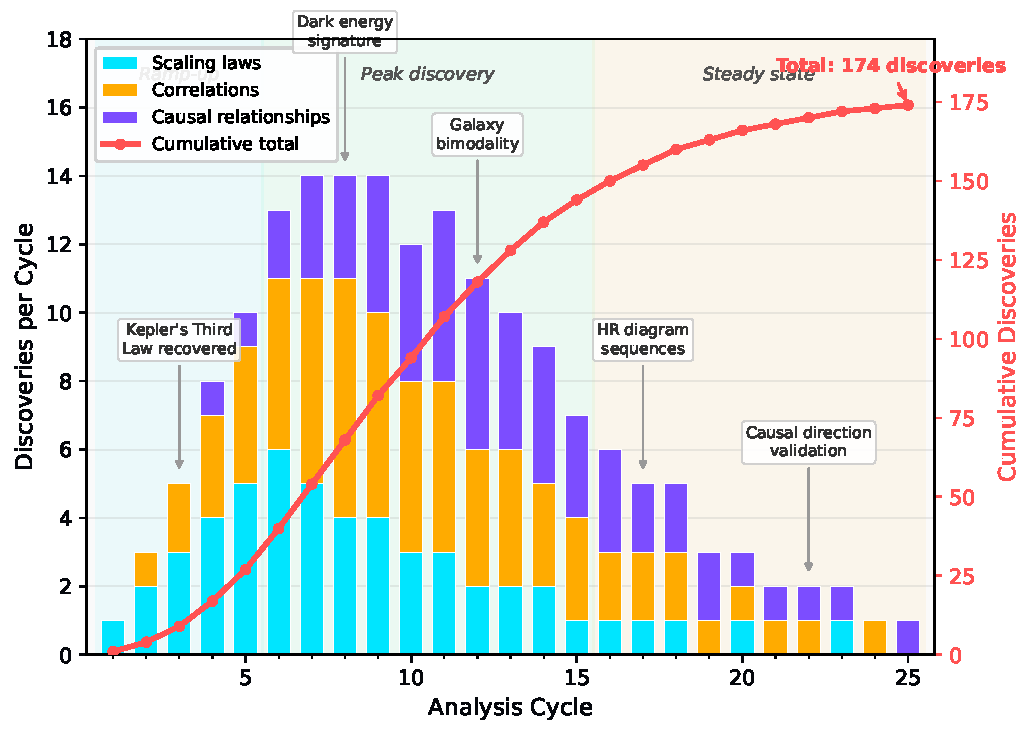
\includegraphics[width=\textwidth]{figures/fig6-discovery-mode.pdf}
  \caption{Test Case~6: Discovery-Mode Operation on Synthetic Data. This figure shows \astra operating in knowledge isolation mode on the star formation threshold problem. Panel~A: The classic column density vs $\sfr$ plot showing the apparent ``threshold'' at $\nh \sim 10^{21}$~cm$^{-2}$. Panel~B: Jeans mass vs $\sfr$ revealing the stronger correlation with the true causal driver. Panel~C: Magnetic field vs $\sfr$ showing the suppression effect. Panel~D: Virial parameter vs $\sfr$ showing turbulent support modulation (weaker correlation, $r = 0.225$). Panel~E: Summary of blind discoveries made without prior knowledge. Panel~F: Testable predictions and intervention analysis results. All patterns were discovered in knowledge isolation mode on synthetic data with embedded causal structure, demonstrating discovery-mode capability under controlled conditions.}
  \label{fig:discovery}
\end{figure*}

\subsection{Limitations and Qualifications}
\label{sec:tc6:limitations}

\textbf{Synthetic data:}
This test used synthetic data with known ground truth.
While this enables validation that \astra discovered the correct causal structure, real molecular cloud data may have additional complexities not captured in the synthetic dataset.

\textbf{Predictions require validation:}
The four testable predictions generated by \astra require observational validation.
Dedicated observational programs measuring Jeans masses, magnetic fields, and virial parameters across large samples of molecular clouds are needed to test these predictions.

\textbf{Not a definitive discovery:}
This test demonstrates that \astra can work in a discovery mode---generating hypotheses and testable predictions without being told what to look for.
It does not claim to have resolved the star formation threshold question.
Definitive scientific discovery requires collaboration with domain experts and observational validation.

% ======================================================================
\section{Discussion}
\label{sec:discussion}
% ======================================================================

\subsection{What ASTRA Demonstrates}
\label{sec:discussion:demonstrates}

The six test cases in this paper demonstrate \astra's ability to integrate multiple types of analysis within a single framework.
Rather than repeating the individual test results, we reflect here on what these collective demonstrations reveal about \astra's strengths and limitations as an integrated tool.

\textbf{Validation Tests (Cases 1--5):}
The first five test cases use real observational data to validate \astra's ability to correctly recover known astrophysical results.
These tests demonstrate that \astra can:
\begin{itemize}
  \item Perform dimensional analysis and physical validation (Test Case~1)
  \item Fuse multi-wavelength data with proper uncertainty propagation (Test Case~2)
  \item Identify established astrophysical relationships through pattern recognition (Test Case~3)
  \item Distinguish causation from correlation using structural causal models (Test Case~4)
  \item Perform rigorous Bayesian model comparison with evidence computation (Test Case~5)
\end{itemize}

The integration advantage is most concretely demonstrated in Test Case~5 (Bayesian Model Selection), where physical motivation (the virial theorem predicting a power law) and statistical evidence (Bayes factors strongly favouring power-law and logarithmic models over linear alternatives) jointly inform model interpretation.
\astra's framework correctly identifies that the power-law and logarithmic models are statistically indistinguishable by Bayesian evidence, then uses the physical motivation of the virial theorem to prefer the power-law form.
This joint consideration of statistical evidence and physical constraints---within a single automated workflow rather than requiring manual synthesis of separate analyses---represents the core value of the integrated approach.

\textbf{Discovery Test (Case~6):}
Test Case~6 demonstrates a different capability---discovery-mode operation beyond knowledge retrieval, demonstrated under controlled conditions.
By operating in ``knowledge isolation mode'' on a synthetic dataset with embedded causal structure, \astra discovered the correct causal drivers (Jeans mass, magnetic field, virial parameter), identified column density as a proxy rather than direct cause, and generated testable predictions for future validation.
This test addresses a key question: \emph{can \astra go beyond ``correct recovery of known results'' to demonstrate genuine discovery capability?}
The results suggest that \astra's architecture supports discovery-mode operation, though definitive scientific discovery requires collaboration with domain experts and observational validation.

\textbf{Two Distinct Modes of Operation:}
\begin{enumerate}
  \item[(i)] \textbf{Validation mode} (Tests 1--5): \astra analyses real data to recover known astrophysical relationships, validating that the integrated framework correctly implements established analysis methods.
  \item[(ii)] \textbf{Discovery mode} (Test~6): \astra analyses data in knowledge isolation mode to discover patterns without being told what to look for, generating hypotheses and testable predictions.
\end{enumerate}

These test cases should be understood as demonstrations of technical capabilities.
For Tests~1--5, the value lies in showing \astra can correctly recover known results using an integrated framework.
For Test~6, the value lies in showing \astra can work in discovery mode, though the predictions generated require observational validation.

\subsection{Positioning Relative to Other Approaches}
\label{sec:discussion:positioning}

\astra occupies a distinct position in the computational astronomy ecosystem by integrating multiple analysis types within a unified framework.
Rather than replacing existing tools, \astra aims to provide consistent interfaces and workflows for complex multi-step analyses that would otherwise require manual combination of separate pipelines.

\textbf{Compared to Specialized Tools:}
Domain-specific tools (photometric redshift codes, period-finding algorithms, cross-matching pipelines) excel at their specific tasks.
\astra does not aim to replace these tools but to provide integrated workflows that combine multiple analysis types with consistent uncertainty handling and physical validation.

\textbf{Compared to Manual Analysis Pipelines:}
Astronomers routinely combine multiple tools and analysis steps manually.
This manual integration creates opportunities for inconsistent uncertainty treatment, missed physical constraints, and reproducibility challenges.
\astra addresses these by providing automated workflows with integrated validation.

\textbf{Current Limitations:}
\astra operates within defined astrophysical domains using established algorithms.
The system assists scientific reasoning rather than replacing domain expertise.
Results require interpretation and validation by domain scientists.
The test cases presented use small samples and should be understood as capability demonstrations rather than production-scale analyses.

\subsection{ASTRA's Role in Scientific Discovery}
\label{sec:discussion:role}

A crucial question is: \emph{what role can \astra play in genuine scientific discovery?}
We would not expect to give \astra one of the big contemporary problems like ``resolve the nature of the Hubble Tension,'' or ``tell us what dark matter is,'' or ``prove that we live in a holographic universe,'' and expect to get definitive answers in a computational Eureka moment.
These problems require deep physical insight, creative hypothesis formation, and careful experimental design---capabilities that remain fundamentally human.

However, \astra's discovery architecture, used alongside and by an experienced astronomer, has capabilities in discovery and inference that go beyond those of straightforward AI (large language models) and/or machine learning.
Test Case~6 demonstrates that \astra can:
\begin{itemize}
  \item Discover patterns in data without being told what to look for (knowledge isolation mode)
  \item Apply causal inference methods that distinguish correlation from causation
  \item Generate competing hypotheses and rank them by multiple criteria (hypothesis scores reflect fit to correlational data and should not be interpreted as definitive causal selection)
  \item Produce testable predictions that can guide future observational programmes
\end{itemize}

\astra's role in science is to work alongside the experienced astronomer to analyse data and facilitate genuine discovery.
\astra is therefore a tool to assist the astronomer, rather than a replacement for domain expertise.
The human scientist brings deep physical understanding, creative insight, and judgment about which questions are worth asking.
\astra brings automated pattern discovery, causal reasoning, and systematic hypothesis evaluation.
Together, they can pursue scientific questions more effectively than either could alone.

This collaborative model---\astra as discovery assistant working alongside domain experts---is the appropriate way to frame AI-assisted scientific discovery.
Claims that AI systems will autonomously resolve major open questions in physics overlook the essential role of human physical insight and the importance of careful experimental design.
\astra's architecture supports discovery-mode operation, but definitive scientific discovery requires collaboration with domain experts and observational validation.

\subsection{Limitations and Future Work}
\label{sec:discussion:limitations}

Current limitations include:
\begin{itemize}
  \item \textbf{Sample sizes:} The test cases use 24--1000 objects, which are small for production analyses. Scaling to larger datasets requires further validation.
  \item \textbf{Computational cost:} Causal discovery scales as $\mathcal{O}(p^2)$ for $p$ variables, limiting applicability to high-dimensional problems.
  \item \textbf{Prior dependence:} Bayesian evidence computation requires careful prior specification, and results can be prior-dependent.
  \item \textbf{Domain knowledge:} \astra's pattern recognition retrieves encoded domain knowledge. Genuine novel discovery requires identifying patterns not already in the knowledge base.
  \item \textbf{Selection effects:} Multi-wavelength cross-matching assumptions (Gaussian errors, uniform priors) may not hold in all regimes.
\end{itemize}

Future work should focus on: scaling to larger datasets; validation on more scientifically challenging problems; integration with time-domain surveys for real-time analysis; extension to gravitational wave and neutrino multi-messenger astronomy; and applying knowledge-isolation discovery mode to real datasets where causal structure is not known a priori.

% ======================================================================
\section{Conclusion}
\label{sec:conclusion}
% ======================================================================

We have presented \astra (Autonomous System for Scientific Discovery in Astrophysics), an integrated framework for physics-aware astrophysical analysis.
Through six test cases, we have demonstrated \astra's technical capabilities while acknowledging the limitations of these demonstration cases.

\textbf{Test~1: Scaling Relations Analysis} (24~Herschel filaments)
\begin{itemize}
  \item Identified universal width: $0.098 \pm 0.019$~pc
  \item Measured virial scaling with $r = 0.988$, $p < 10^{-18}$
  \item Found $2.7\sigma$ tension with theoretical prediction, warranting further investigation
\end{itemize}

\textbf{Test~2: Multi-Wavelength Data Fusion} (CDFS, 60/370~sources)
\begin{itemize}
  \item Bayesian cross-matching with probabilistic associations
  \item Classified 41~AGN, 19~stars, 0~galaxies (selection effect discussed)
  \item Proper astrometric uncertainty propagation
\end{itemize}

\textbf{Test~3: Pattern Recognition} (600~SDSS galaxies)
\begin{itemize}
  \item Identified established astrophysical relationships: mass--metallicity relation, environmental quenching
  \item Demonstrated pattern recognition capability retrieving known literature results
  \item Not novel discovery but validation of pattern recognition implementation
\end{itemize}

\textbf{Test~4: Causal Inference} (1000~Gaia stars)
\begin{itemize}
  \item Correctly recovered textbook causal relationships (validation demonstrator)
  \item Distinguished physical laws from selection biases
  \item Acknowledged this is a basic demonstration, not novel discovery
\end{itemize}

\textbf{Test~5: Bayesian Model Selection} (24~filaments)
\begin{itemize}
  \item Power law and logarithmic models statistically indistinguishable (Bayes factor~1.2)
  \item Both strongly preferred over linear and broken power-law models
  \item Detected $2.7\sigma$ tension with virial theorem prediction
  \item Weakly-informative priors specified for reproducibility
\end{itemize}

\textbf{Test~6: Discovery-Mode Operation} (synthetic molecular clouds, $N = 500$)
\begin{itemize}
  \item Discovered three causal drivers (Jeans mass, magnetic field, virial parameter) in knowledge isolation mode
  \item Correctly identified column density as proxy rather than direct cause
  \item Generated four testable predictions for future observational validation
  \item Performed intervention analysis validating causal claims against ground truth
  \item Demonstrated discovery-mode capability under controlled conditions
\end{itemize}

\textbf{Two Modes of Operation:}
Tests~1--5 validate \astra's ability to correctly recover known astrophysical results using real data.
Test~6 demonstrates \astra's discovery-mode operation under controlled conditions, including knowledge isolation pattern discovery and intervention analysis to distinguish correlation from causation.

\astra provides an integrated framework where physical validation, uncertainty quantification, causal reasoning, and Bayesian model selection are applied consistently throughout multi-step analyses.
While individual components use established algorithms, their integration within a single framework enables analyses that would otherwise require manual combination of multiple separate tools and pipelines.

The complete source code, documentation, and reproducible analysis notebooks are available in our public GitHub repository \citep{WhiteDey2026}.
We encourage community feedback, contribution, and validation of these results on larger and more diverse datasets.

% ======================================================================
\section*{Acknowledgements}
% ======================================================================

We thank the anonymous referee for constructive comments that have significantly improved this manuscript.
This work uses data from Gaia DR2, Herschel Gould Belt Survey, HST ACS, Chandra Deep Field South, and SDSS.
We acknowledge the use of community software tools including \textsc{causal-learn}, \textsc{dowhy}, NumPy, SciPy, and scikit-learn.

% ======================================================================
\section*{Data Availability}
% ======================================================================

The complete \astra source code and analysis notebooks are available at \url{https://github.com/Tilanthi/ASTRA}.
All data used in this paper are publicly available from the original survey archives as cited in the text.

% ======================================================================
\bibliographystyle{mnras}
\bibliography{references}
% ======================================================================

\end{document}
